\section{Cart-pole Balance via Reinforcement Learning}

\subsection*{(a)}
% I used a three-layer MLP to map the CartPole state to two
% Q-values, one for each action. During training the policy uses epsilon-greedy
% exploration, and during evaluation it picks the action with the largest Q-value.
% The replay-buffer update uses the usual Bellman target
% \[
% r+\gamma\max_{a'}Q(s',a')
% \]
% and minimizes the squared error between the selected Q-value and this target.

\textbf{(i) build\_network}
\begin{lstlisting}[language=Python]
return torch.nn.Sequential(
    torch.nn.Linear(self.state_dim, self.hidden_dim),
    torch.nn.ReLU(),
    torch.nn.Linear(self.hidden_dim, self.hidden_dim),
    torch.nn.ReLU(),
    torch.nn.Linear(self.hidden_dim, self.action_dim),
)
\end{lstlisting}

\textbf{(ii) policy}
\begin{lstlisting}[language=Python]
if train and random.random() < self.eps_threshold():
    return torch.randint(self.action_dim, (1,), device=self.device)

with torch.no_grad():
    q_values = self.policy_network(state)
    return torch.argmax(q_values, dim=-1)
\end{lstlisting}

\textbf{(iii) train}
\begin{lstlisting}[language=Python]
optimizer = torch.optim.AdamW(self.policy_network.parameters(), lr=self.learning_rate)
loss_fn = torch.nn.MSELoss()

for _ in tqdm(range(num_episodes)):
    obs, info = env.reset()
    state = torch.tensor(obs, dtype=torch.float32).unsqueeze(0).to(self.device)
    terminated, truncated = False, False

    while not terminated and not truncated:
        action = self.policy(state, train=True)
        obs, reward, terminated, truncated, info = env.step(action.item())

        reward = torch.tensor([reward], dtype=torch.float32).to(self.device)
        next_state = None
        if not terminated and not truncated:
            next_state = torch.tensor(obs, dtype=torch.float32).unsqueeze(0).to(self.device)

        self.buffer.append(Transition(state, action, reward, next_state))
        state = next_state

        if len(self.buffer) > self.batch_size:
            states, actions, targets = self.sample_buffer()
            q_values = self.policy_network(states).gather(1, actions)
            loss = loss_fn(q_values, targets)

            optimizer.zero_grad()
            loss.backward()
            torch.nn.utils.clip_grad_value_(self.policy_network.parameters(), 100)
            optimizer.step()
\end{lstlisting}

\textbf{(iv) Training results}

Using 10 evaluation rollouts, the randomly initialized DQN policy had
\begin{lstlisting}
--- Reward Statistics ---
Average: 9.4
Standard deviation: 0.9165151389911681
Minimum: 8.0
Maximum: 11.0
\end{lstlisting}

After 100 training episodes, the evaluated policy had
\begin{lstlisting}
--- Reward Statistics ---
Average: 9.7
Standard deviation: 0.6403124237432849
Minimum: 9.0
Maximum: 11.0
\end{lstlisting}
% In this run, DQN improved only slightly. This is not too surprising: the run is
% short, and the learned Q-values were still not strong enough to produce a much
% better greedy policy.

\subsection*{(b)}
% For REINFORCE, I implemented the three policy-gradient estimators requested in
% the problem: the naive full-trajectory return, the causality-trick return, and
% the causality-trick return with an average-return baseline.

\textbf{(i) Naive policy gradient}
\begin{lstlisting}[language=Python]
# 1) Naive REINFORCE
discounted_return = torch.tensor(
    sum((self.gamma ** t) * rewards[t] for t in range(len(rewards))),
    dtype=torch.float,
)
naive_loss = -torch.stack(
    [log_prob * discounted_return for log_prob in log_probs]
).sum()

# 2) REINFORCE with causality trick
returns = []
running_return = 0.0
for reward in reversed(rewards):
    running_return = reward + self.gamma * running_return
    returns.insert(0, running_return)
returns = torch.tensor(returns, dtype=torch.float)
causal_loss = -torch.stack(
    [log_prob * ret for log_prob, ret in zip(log_probs, returns)]
).sum()

# 3) REINFORCE with causality trick and baseline to "center" the returns
baseline = returns.mean()
baseline_loss = -torch.stack(
    [log_prob * (ret - baseline) for log_prob, ret in zip(log_probs, returns)]
).sum()

if self.gradient_variant == "naive":
    loss = naive_loss
elif self.gradient_variant == "causal":
    loss = causal_loss
else:
    loss = baseline_loss
\end{lstlisting}

\textbf{(iv) Training results}

\begin{figure}[H]
\centering
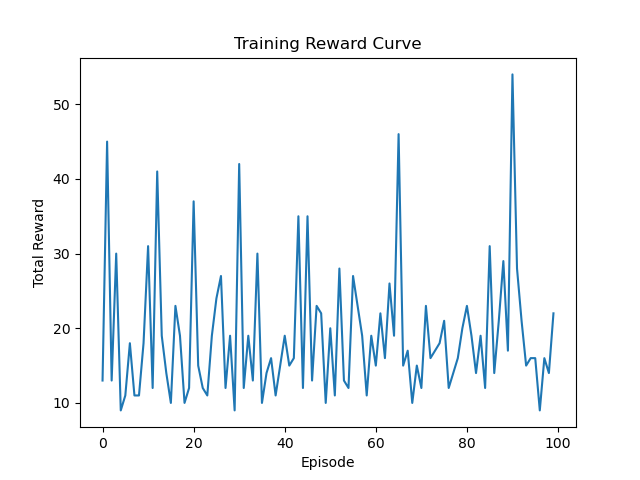
\includegraphics[width=0.32\textwidth]{figures/reinforce_naive_rewards.png}
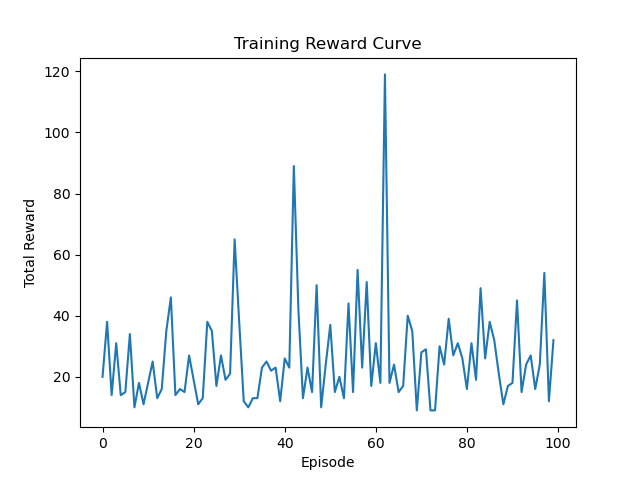
\includegraphics[width=0.32\textwidth]{figures/reinforce_causal_rewards.png}
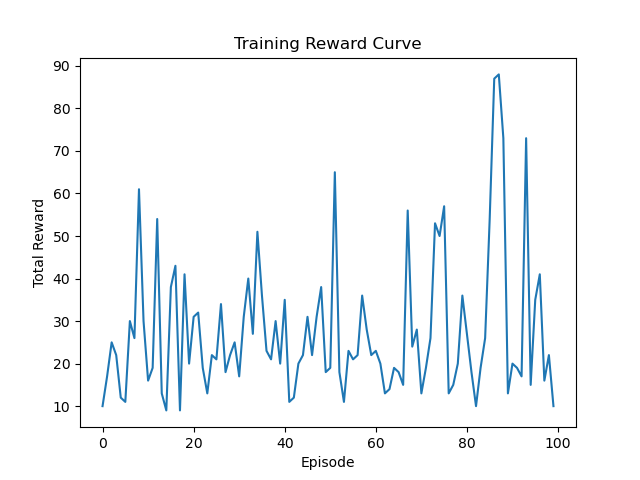
\includegraphics[width=0.32\textwidth]{figures/reinforce_baseline_rewards.png}
\caption{REINFORCE reward curves for naive, causal, and baseline variants}
\label{fig:reinforce_rewards}
\end{figure}

\begin{lstlisting}
--- Reward Statistics ---
Average: 152.7
Standard deviation: 54.30478800253251
Minimum: 86.0
Maximum: 248.0
\end{lstlisting}

Compared with the DQN run above, REINFORCE performed much better after training.
The reward curve is still noisy because policy-gradient updates use sampled
trajectories directly, but the baseline estimator helps reduce variance by
centering the returns.
